\documentclass{article}
\usepackage[utf8]{inputenc}
\usepackage{tikz,graphicx,hyperref,amsmath,amsfonts,amscd,amssymb,bm,cite,epsfig,epsf,url}

\title{big data quiz 1 }
\author{wbg231 }
\date{January 2023}

\begin{document}

\maketitle

\section{Introduction}
\begin{itemize}
    \item a table in a relational database must have exactly one index 
    \item that is false there are foreign keys 
    \item each table in a relational database must have a primary key 
    \item this is false  ( i am not sure the purpose of not having a primary key but that is something you can do)
    \item in a relational data base a primary key value must be unique across all tables in the database 
    \item i think false, just has to be true when you join like one user can have multiple songs they like in recommender systems
    \item 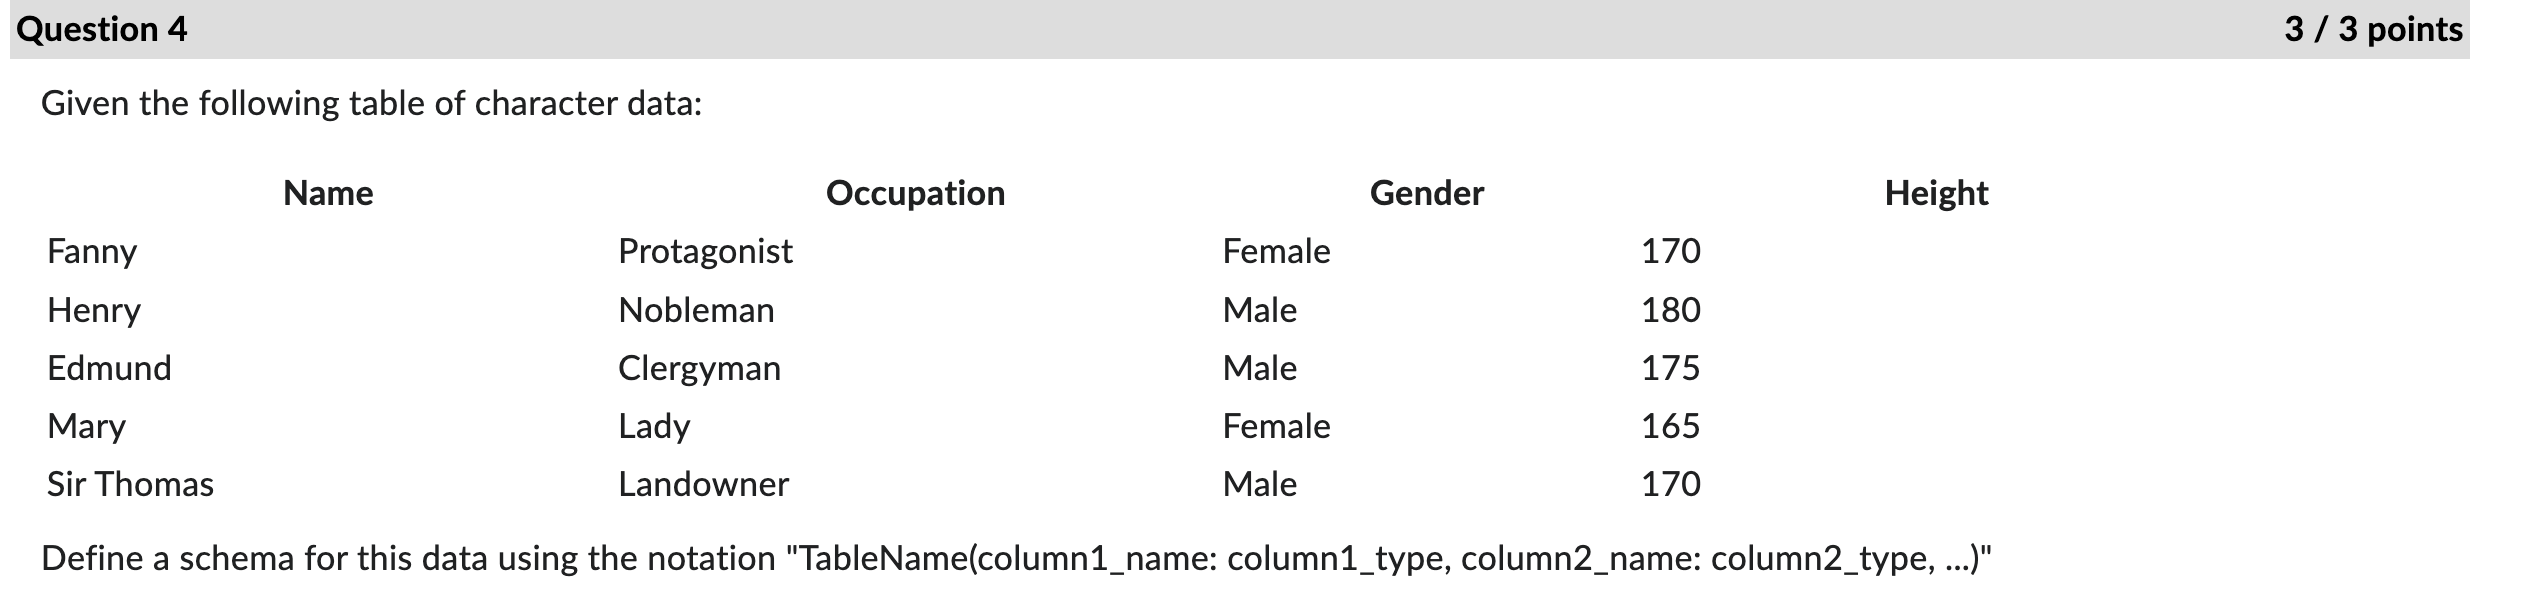
\includegraphics{/Users/hochwagenlab/Desktop/buz/school/big-data-spring-2023/review/week_2/quiz_1/images/Screenshot 2023-05-08 at 3.57.27 PM.png}
    \item characters(name: STR, occupation : str, gender : STR, Height: int)
    \item 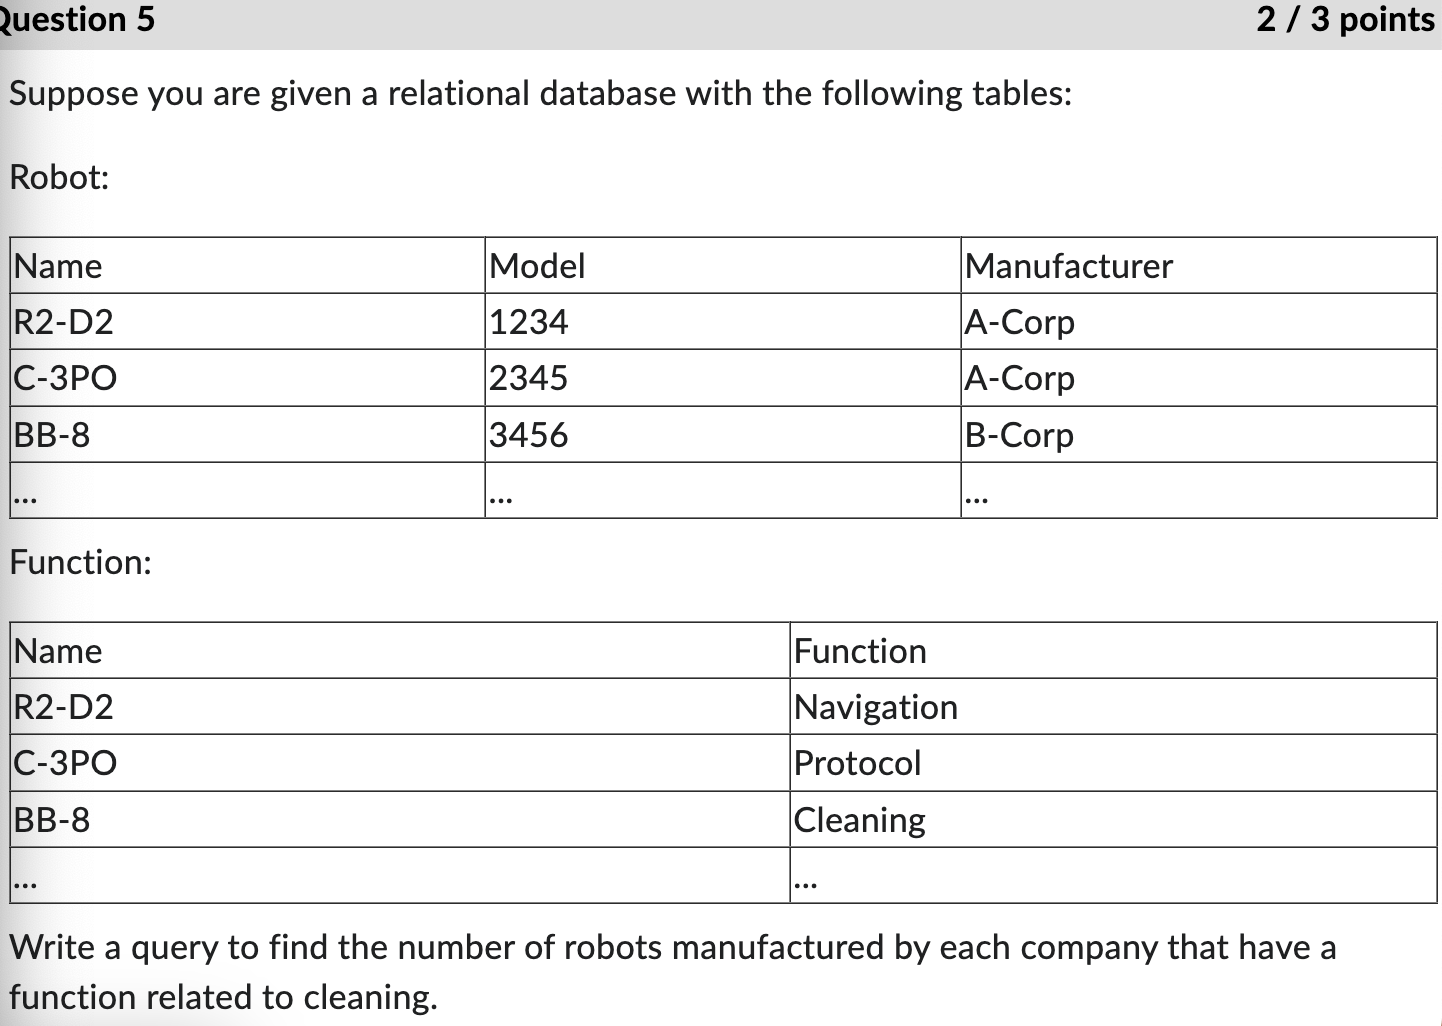
\includegraphics{images/Screenshot 2023-05-08 at 4.01.12 PM.png}
    \item select count(names) from robot left join function on robot.name = function.name where function.function="Cleaning" group by robot.manufacturer
\end{itemize}
\end{document}
